
\documentclass[12pt]{report}

%EndMSIPreambleData
\providecommand{\U}[1]{\protect\rule{.1in}{.1in}}
\pretolerance=10000
\baselineskip=9.in
\evensidemargin 0.0 in
\oddsidemargin 0.0 in
\parindent 24pt
\textheight 8.5 in
\textwidth 6.5 in
\topmargin -0.5 in
\renewcommand{\baselinestretch}{1.18} %% Packages
\usepackage{amssymb,amsthm,amsfonts,amsmath,pifont}
\usepackage{enumerate}
\usepackage[brazil]{babel}
\usepackage[latin1]{inputenc}
\usepackage{hyperref}
\usepackage{dsfont}
\usepackage{upgreek}
\usepackage{graphicx}
\usepackage{indentfirst}%1ª linha do capitulo em paragrafo%
\setcounter{MaxMatrixCols}{30}
\usepackage{color}
\usepackage{float}

%\usepackage[applemac]{inputenc}
%\usepackage[portuges,brazilian]{babel}
%\usepackage[T1]{fontenc}

\begin{document}
\thispagestyle{empty}

\begin{figure}[ht]
\hspace{0.5cm}
\begin{minipage}[b]{0.11\linewidth}
\centering

\includegraphics[width=1.5cm]{logoufpe.jpg}
\end{minipage}
\hspace{0.5cm}
\begin{minipage}[b]{0.75\linewidth}
\centering
\large\textbf{Universidade Federal de Pernambuco}\\
Centro Acad\^emico do Agreste	\\
N\'ucleo de Forma\c{c}\~ao Docente\\
\end{minipage}
\end{figure}
Professor: \textbf{Felipe Trajano}
\vspace{0.2cm}

Aluno: \_\_\_\_\_\_\_\_\_\_\_\_\_\_\_\_\_\_\_\_\_\_\_\_\_\_\_\_\_\_\_\_\_\_\_\_\_\_\_\_\_\_\_\_\_\_\_\_\_\_\_\_\_\_\_\_\_\_\_\_\_\_\_\_\_\_\_\_ Nota: \_\_\_\_\_\_\_\_\_\_\_\_
\vspace{0.2cm}
\begin{center}
\textbf{Avalia\c{c}\~ao}
\end{center}


\vspace{0.2cm}
\normalsize

\begin{enumerate}

%-----------------PRIMEIRA QUESTÌO-----------------------------------------
\item 
Na teoria das elei��es, o M�todo de Borda sugere que, em vez de escolher um candidato, cada juiz deve criar um ranking de sua prefer�ncia para os concorrentes (isto �, criar uma lista com a ordem de classifica��o dos concorrentes). A este ranking � associada uma pontua��o: um ponto para o �ltimo colocado no ranking, dois pontos para o pen�ltimo, tr�s para o antepen�ltimo, e assim sucessivamente. Ao final, soma-se a pontua��o atribu�da a cada concorrente por cada um dos ju�zes. 
Em uma escola houve um concurso de poesia no qual cinco alunos concorreram a um pr�mio, sendo julgados por 25 ju�zes. Para a escolha da poesia vencedora foi utilizado o M�todo de Borda. Nos quadros, est�o apresentados os rankings dos ju�zes e a frequ�ncia de cada ranking. 

\begin{figure}[h]
\centering
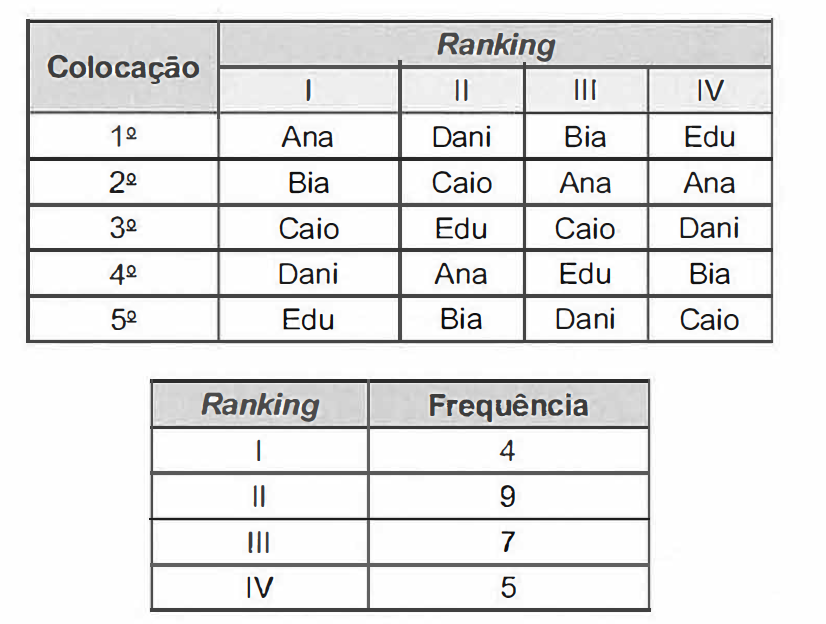
\includegraphics[width=8cm]{../figuras/q141-2018.png}
\end{figure}

\begin{enumerate}
\item[a)]Edu.
\item[b)]Dani.
\item[c)]Caio.
\item[d)]Bia
\item[e)]Ana.
\end{enumerate}

%------------------SEGUNDA QUESTÌO------------------------------------------
\newpage
\item 
A inclina��o de uma rampa � calculada da seguinte maneira: para cada metro medido na horizontal, mede-se x cent�metros na vertical. Diz-se, nesse caso, que a rampa tem inclina��o de x\%, como no exemplo da figura: 

\begin{figure}[h]
\centering
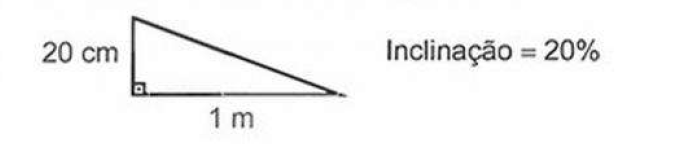
\includegraphics[width=8cm]{../figuras/q172(1)-2018.png}
\end{figure}

A figura apresenta um projeto de uma rampa de acesso a uma garagem residencial cuja base, situada 2 melros abaixo do n�vel da rua, tem 8 metros de comprimento. 

\begin{figure}[h]
\centering
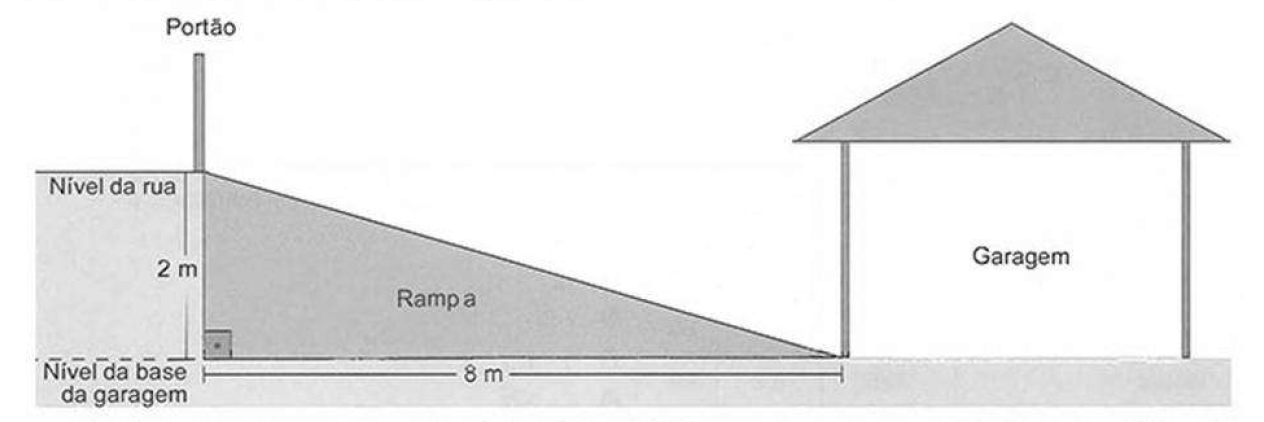
\includegraphics[width=8cm]{../figuras/q172(2)-2018.png}
\end{figure}

Depois de projetada a rampa, o respons�vel pela obra foi informado de que as normas t�cnicas do munic�pio onde ela est� localizada exigem que a inclina��o m�xima de uma rampa de acesso a uma garagem residencial seja de 20\%. 
Se a rampa projetada tiver inclina��o superior a 20\%, o n�vel da garagem dever� ser alterado para diminuir o percentual de inclina��o. mantendo o comprimento da base da rampa. 
Para atender �s normas t�cnicas do munic�pio, o n�vel da garagem dever� ser 

\begin{enumerate}
\item[a)]elevado em 40 cm
\item[b)] elevado em 50 cm 
\item[c)] mantido no mesmo n�vel
\item[d)] rebaixado em 40 cm 
\item[e)] rebaixado em 50 cm
\end{enumerate}

%----------------TERCEIRA QUESTÌO--------------------------------------------
\newpage
\item 
O colesterol total de uma pessoa � obtido pela soma da taxa do seu "colesterol bom" com a taxa do seu "colesterol ruim". Os exames peri�dicos, realizados em um paciente adulto, apresentaram taxa normal de "colesterol bom", por�m, taxa do "colesterol ruim" (tamb�m chamado LDL) de 280 mg/dl. 
O quadro apresenta uma classifica��o de acordo com as taxas de LDL em adultos. 

\begin{figure}[h]
\centering
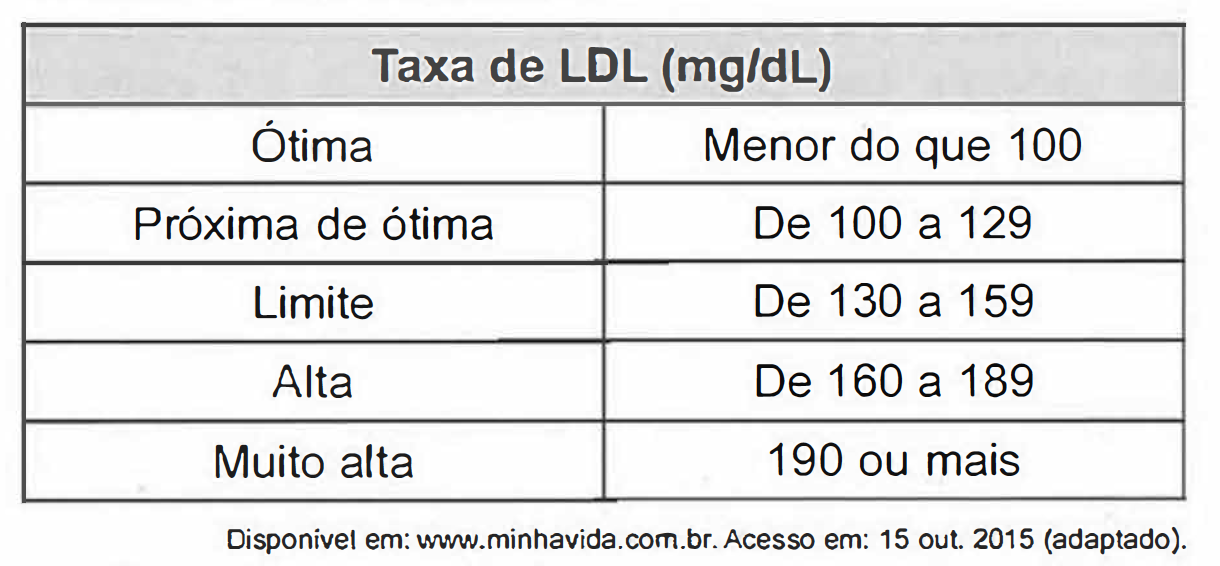
\includegraphics[width=8cm]{../figuras/q163-2018.png}
\end{figure}

O paciente, seguindo as recomenda��es m�dicas sobre estilo de vida e alimenta��o, realizou o exame logo ap�s o primeiro m�s, e a taxa de LDL reduziu 25\%. No m�s seguinte, realizou novo exame e constatou uma redu��o de mais 20\% na taxa de LDL. 
De acordo com o resultado do segundo exame, a classifica��o da taxa de LDL do paciente � 

\begin{enumerate}
\item[a)]�tima
\item[b)]pr�xima de �tima.
\item[c)]limite.
\item[d)]alta.
\item[e)]muito alta
\end{enumerate}

%-----------------QUINTA QUESTÌO-----------------------------------------------
\newpage
\item     
Minecraft � um jogo virtual que pode auxiliar no desenvolvimento de conhecimentos relacionados a espa�o e forma. � poss�vel criar casas, edif�cios, monumentos e at� naves espaciais, tudo em escala real, atrav�s do empilhamento de cubinhos. 
Um jogador deseja construir um cubo com dimens�es 4 x 4 x 4. Ele j� empilhou alguns dos cubinhos necess�rios. conforme a figura. 

\begin{figure}[h]
\centering
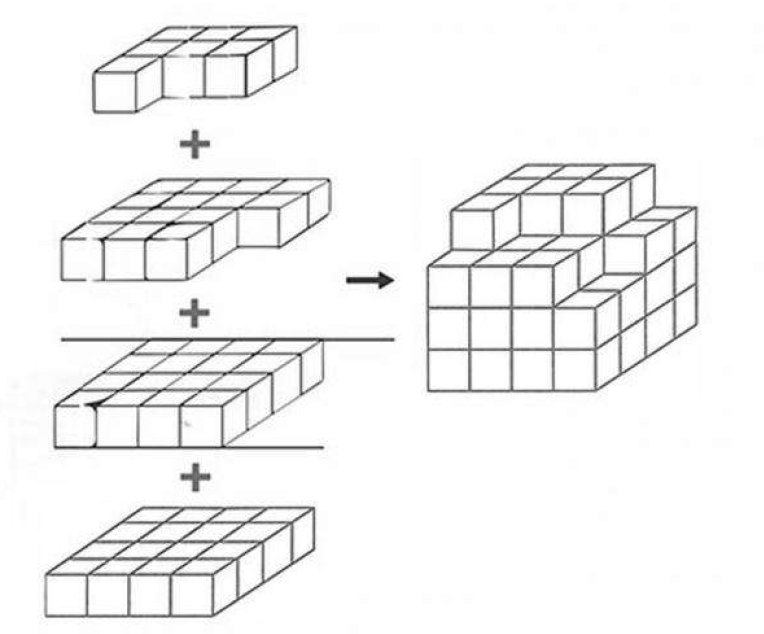
\includegraphics[width=8cm]{../figuras/q169(1)-2018}
\end{figure}

Os cubinhos que ainda faltam empilhar para finalizar a constru��o do cubo. juntos, formam uma pe�a �nica, capaz de completar a tarefa. 
O formato da pe�a capaz de completar o cubo 4 x 4 x 4 � 

\begin{figure}[h]
\centering
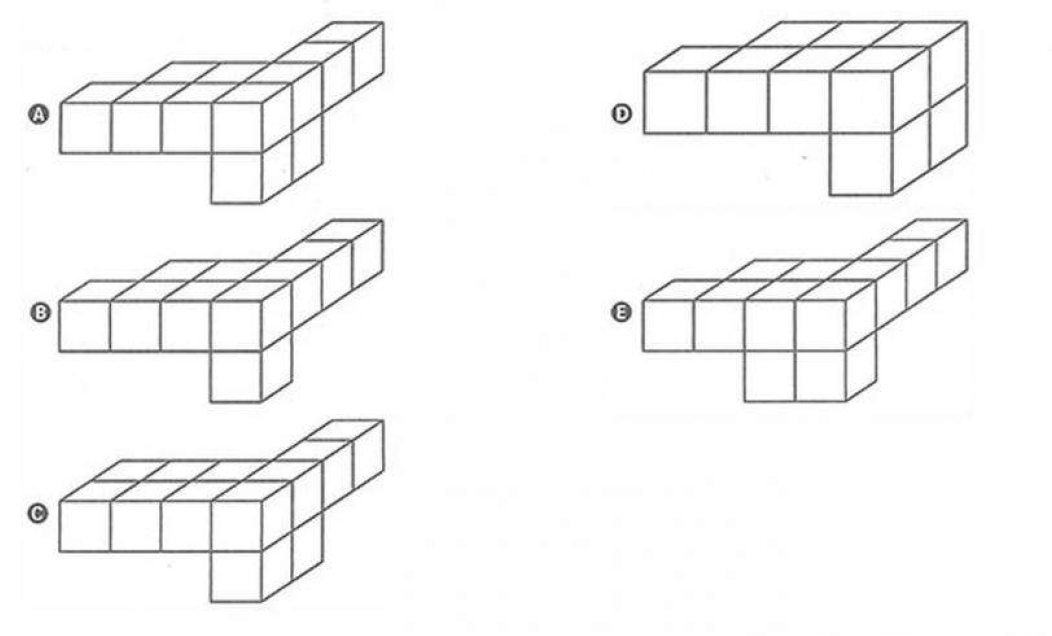
\includegraphics[width=8cm]{../figuras/q169(2)-2018.png}
\end{figure}

\begin{enumerate}
\item[a)]a
\item[b)]b
\item[c)]c
\item[d)]d
\item[e)]e
\end{enumerate}


%----------------QUARTA QUESTÌO---------------------------------------------
\newpage
\item 
A figura mostra uma pra�a circular que cont�m um chafariz em seu centro e, em seu entorno, um passeio. Os c�rculos que definem a pra�a e o chafariz s�o conc�ntricos. 

\begin{figure}[h]
\centering
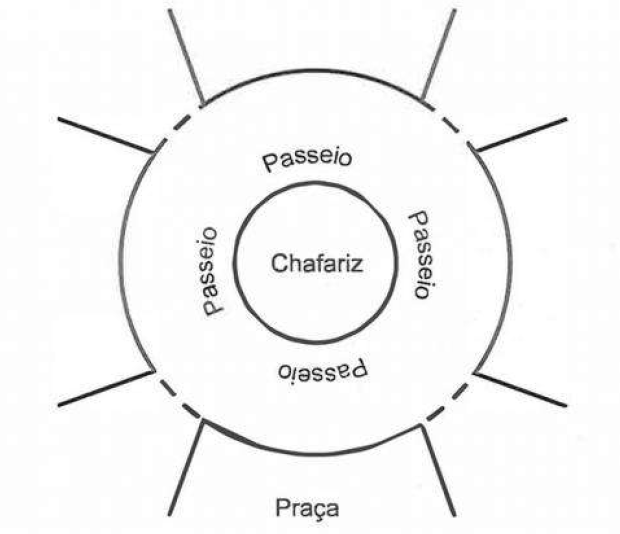
\includegraphics[width=8cm]{../figuras/q170(1)-2018.png}
\end{figure}

O passeio ter� seu piso revestido com ladrilhos. Sem condi��es de calcular os raios, pois o chafariz est� cheio, um engenheiro fez a seguinte medi��o: esticou uma trena tangente ao chafariz, medindo a dist�ncia entre dois pontos A e 8, conforme a figura. Com isso, obteve a medida do segmento de reta AB: 16 m. 


\begin{figure}[h]
\centering
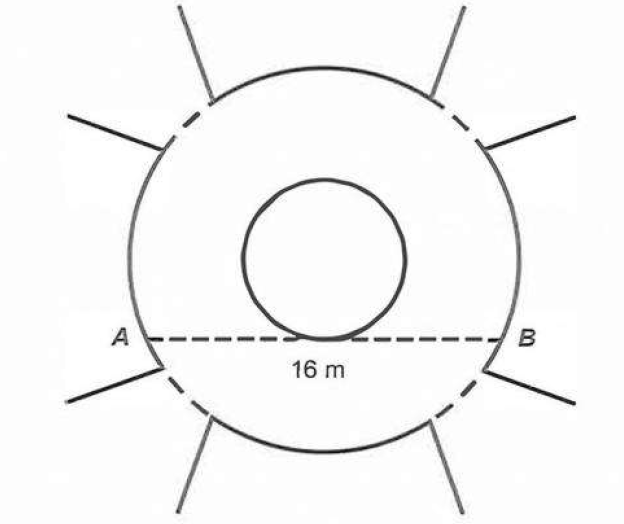
\includegraphics[width=8cm]{../figuras/q170(2)-2018.png}
\end{figure}

Dispondo apenas dessa medida, o engenheiro calculou corretamente a medida da �rea do passeio, em metro quadrado. 
A medida encontrada pelo engenheiro foi:
\newline
\\
$a)4\pi\quad b)8\pi\quad c)48\pi\quad d)64\pi\quad e)192\pi$


\end{enumerate}
\end{document}

